\documentclass[aspectratio=169, 11pt]{beamer}

% ------------------------------------------------
% Estilo: sobrio, mismos colores que las figuras del proyecto
% ------------------------------------------------
\usepackage{graphicx}
\usepackage{booktabs}
\graphicspath{{../../outputs/figuras/}}

\definecolor{azul}{HTML}{2A78D6}
\definecolor{naranja}{HTML}{EB6834}
\definecolor{tinta}{HTML}{2B2B29}
\definecolor{suave}{HTML}{6B6A65}
\setbeamercolor{frametitle}{fg=tinta}
\setbeamercolor{title}{fg=tinta}
\setbeamercolor{normal text}{fg=tinta}
\setbeamercolor{structure}{fg=azul}
\setbeamercolor{alerted text}{fg=naranja}
\setbeamerfont{frametitle}{series=\bfseries}
\setbeamertemplate{navigation symbols}{}
\setbeamertemplate{itemize items}[circle]
\setbeamertemplate{footline}{\hfill\color{suave}\scriptsize\insertframenumber\hspace{1.2em}\vspace{0.8em}}

\title{Vulnerabilidad de la red vial primaria de carga de Colombia}
\subtitle{Una evaluación con teoría de grafos}
\author{David Catral \and Gabriel Salcedo \and Isaac Suárez}
\institute{Teoría de Grafos · Universidad del Rosario}
\date{2026-II}

\begin{document}

% 1 ------------------------------------------------
\begin{frame}
  \titlepage
\end{frame}

% 2 ------------------------------------------------
\begin{frame}{El problema}
  \begin{itemize}
    \item La carga del país se mueve por carretera, sobre pocos corredores troncales.
    \item Derrumbes, bloqueos y obras cierran esos corredores con frecuencia.
    \item Cada cierre obliga a desviar la carga: más km, más flete, o ninguna ruta.
  \end{itemize}
  \vspace{1.2em}
  \begin{block}{Pregunta}
    ¿Qué tramos causan el mayor daño económico cuando se cierran?\\[0.3em]
    \small (a) sobrecosto en pesos de la carga que se desvía \quad
    (b) toneladas que se quedan sin ruta
  \end{block}
\end{frame}

% 3 ------------------------------------------------
\begin{frame}{Hipótesis: tres ángulos que no coinciden}
  \begin{columns}[T]
    \column{0.32\textwidth}\centering
      {\Large\bfseries\color{azul}Posición}\\[0.4em]
      intermediación $C_B(e)$\\[0.2em]
      \small ¿cuántas parejas de ciudades pasan por aquí?
    \column{0.32\textwidth}\centering
      {\Large\bfseries\color{azul}Uso}\\[0.4em]
      carga asignada $x_e$\\[0.2em]
      \small ¿cuántas toneladas pasan de verdad?
    \column{0.32\textwidth}\centering
      {\Large\bfseries\color{naranja}Consecuencia}\\[0.4em]
      sobrecosto $I(e)$ y carga sin ruta $D(e)$\\[0.2em]
      \small ¿cuánto cuesta perderlo?
  \end{columns}
  \vspace{2em}
  \centering
  Si coincidieran, bastaría con mirar el mapa.\\
  \alert{En las diferencias están los tramos subestimados.}
\end{frame}

% 4 ------------------------------------------------
\begin{frame}{Datos y modelo}
  \begin{columns}[T]
    \column{0.5\textwidth}
      \textbf{Datos públicos}
      \begin{itemize}\small
        \item Red vial INVIAS (HDX): 652 tramos, 20.011 km
        \item RNDC 2015: matriz origen--destino de toneladas
        \item DIVIPOLA (DANE): ubicación de municipios
      \end{itemize}
      \vspace{0.6em}
      \textbf{Peso de cada arista}
      \[ w_{uv} = 248{,}6\ \tfrac{\text{COP}}{\text{t-km}} \times \ell_{uv} \]
      \small costo de mover una tonelada por el corredor
    \column{0.5\textwidth}
      \textbf{Del mapa al grafo}
      \begin{itemize}\small
        \item Limpieza: 464 $\to$ 22 componentes
        \item Red detallada $D$: 842 nodos, 972 aristas
        \item Grafo de análisis $G$: \alert{25 ciudades + 28 cruces, 77 aristas}
        \item $G$ simple, no dirigido, conexo y planar
        \item La dirección de la carga vive en la matriz $T$
      \end{itemize}
  \end{columns}
\end{frame}

% 5 ------------------------------------------------
\begin{frame}{El grafo de análisis}
  \begin{columns}[c]
    \column{0.45\textwidth}\centering
      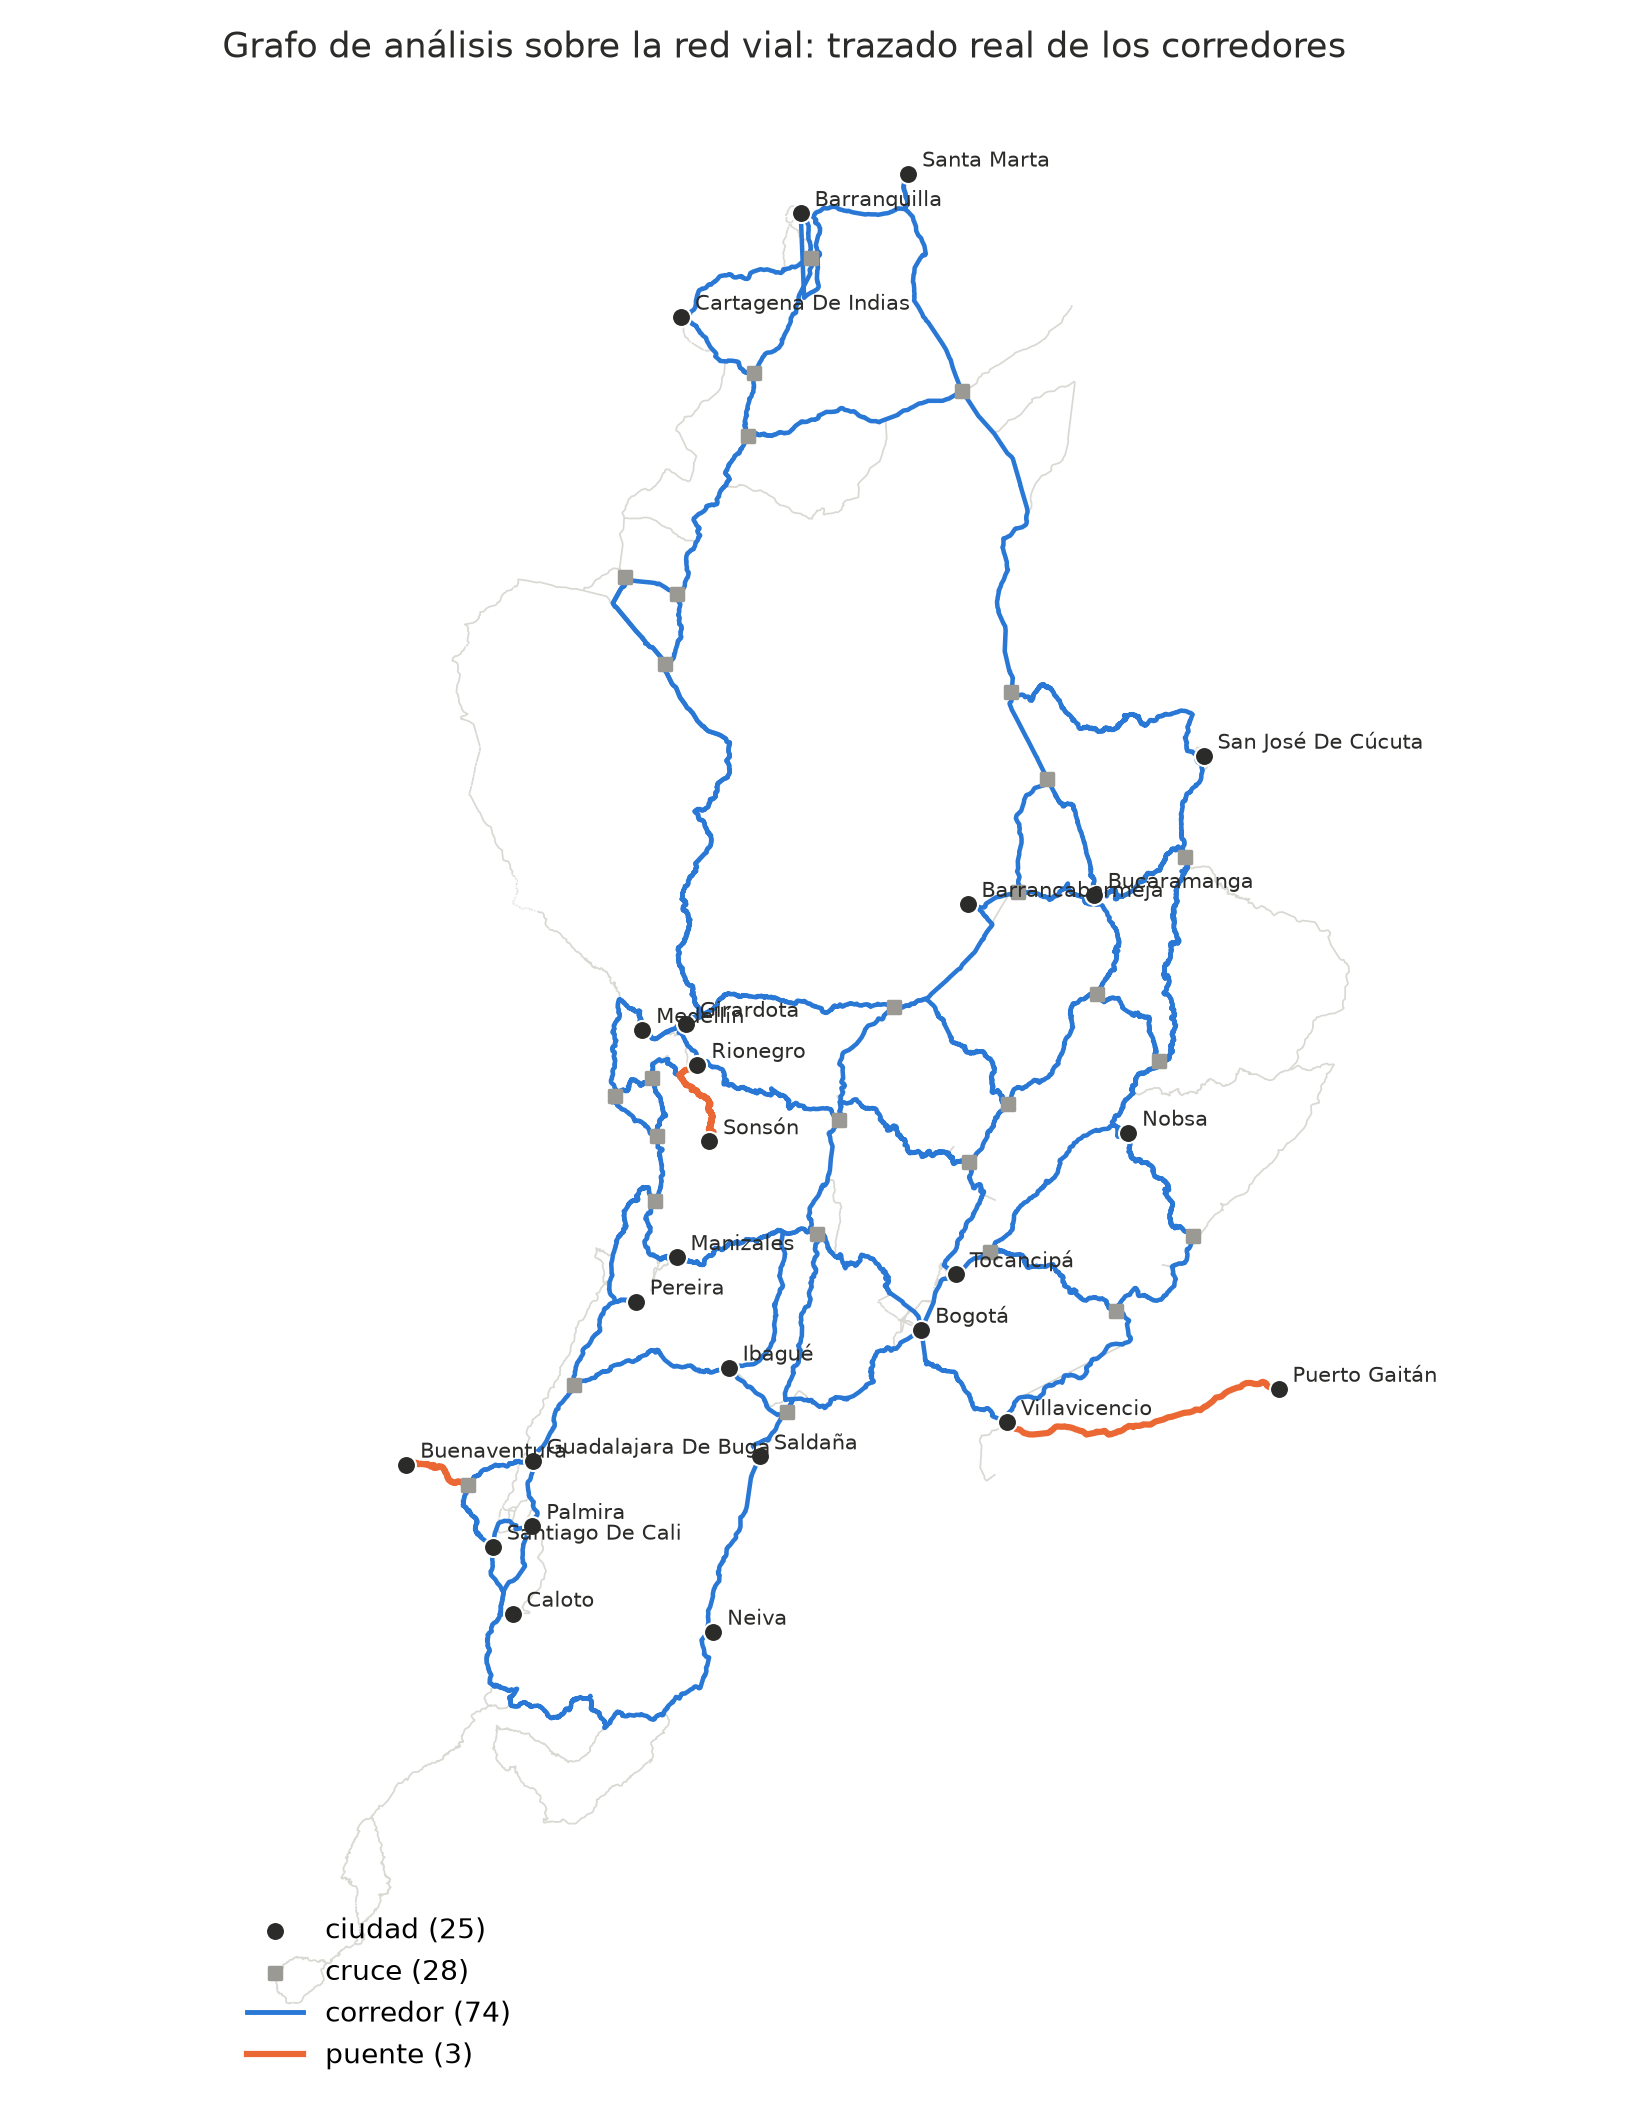
\includegraphics[height=0.82\textheight]{grafo_analisis_mapa.png}
    \column{0.55\textwidth}
      \begin{itemize}
        \item $\kappa(G) = \lambda(G) = 1$: \alert{una sola falla parte la red}
        \item 3 puentes (naranja): Buenaventura--Dagua, Villavicencio--Puerto Gaitán,
              Rionegro--Sonsón
        \item Diámetro: 14 aristas; grado medio 2,91
        \item Validación: km del grafo / km del RNDC = 1,04 (300 parejas con más carga)
      \end{itemize}
  \end{columns}
\end{frame}

% 6 ------------------------------------------------
\begin{frame}{Implementación}
  \begin{columns}[T]
    \column{0.55\textwidth}
      \begin{itemize}\small
        \item \textbf{Dijkstra propio} (montículo binario): rutas más baratas;
              igual a NetworkX en 200 parejas
        \item \textbf{Asignación todo o nada}: $x_e$ = intermediación ponderada por toneladas
        \item \textbf{Brandes}: intermediación entre las 25 ciudades
        \item \textbf{Tarjan}: puentes y vértices de corte
        \item \textbf{Algoritmo de cierres}: se quita $e$, se recalcula, se mide $I$ y $D$\\
              77 aristas + 243 tramos de INVIAS, en 3 segundos
      \end{itemize}
    \column{0.42\textwidth}
      \begin{block}{Daño de cerrar $e$}
        \[ I(e) = \sum_{\text{con ruta}} T_{od}\,\big[c_{G-e} - c_G\big] \]
        \[ D(e) = \sum_{\text{sin ruta}} T_{od} \]
      \end{block}
      \vspace{0.4em}
      \small 9 de 9 pruebas con respuestas calculadas a mano.\\
      Todo el proceso es reproducible en 2,5 minutos.
  \end{columns}
\end{frame}

% 7 ------------------------------------------------
\begin{frame}{Resultado 1: la posición no es el uso}
  \begin{columns}[c]
    \column{0.58\textwidth}\centering
      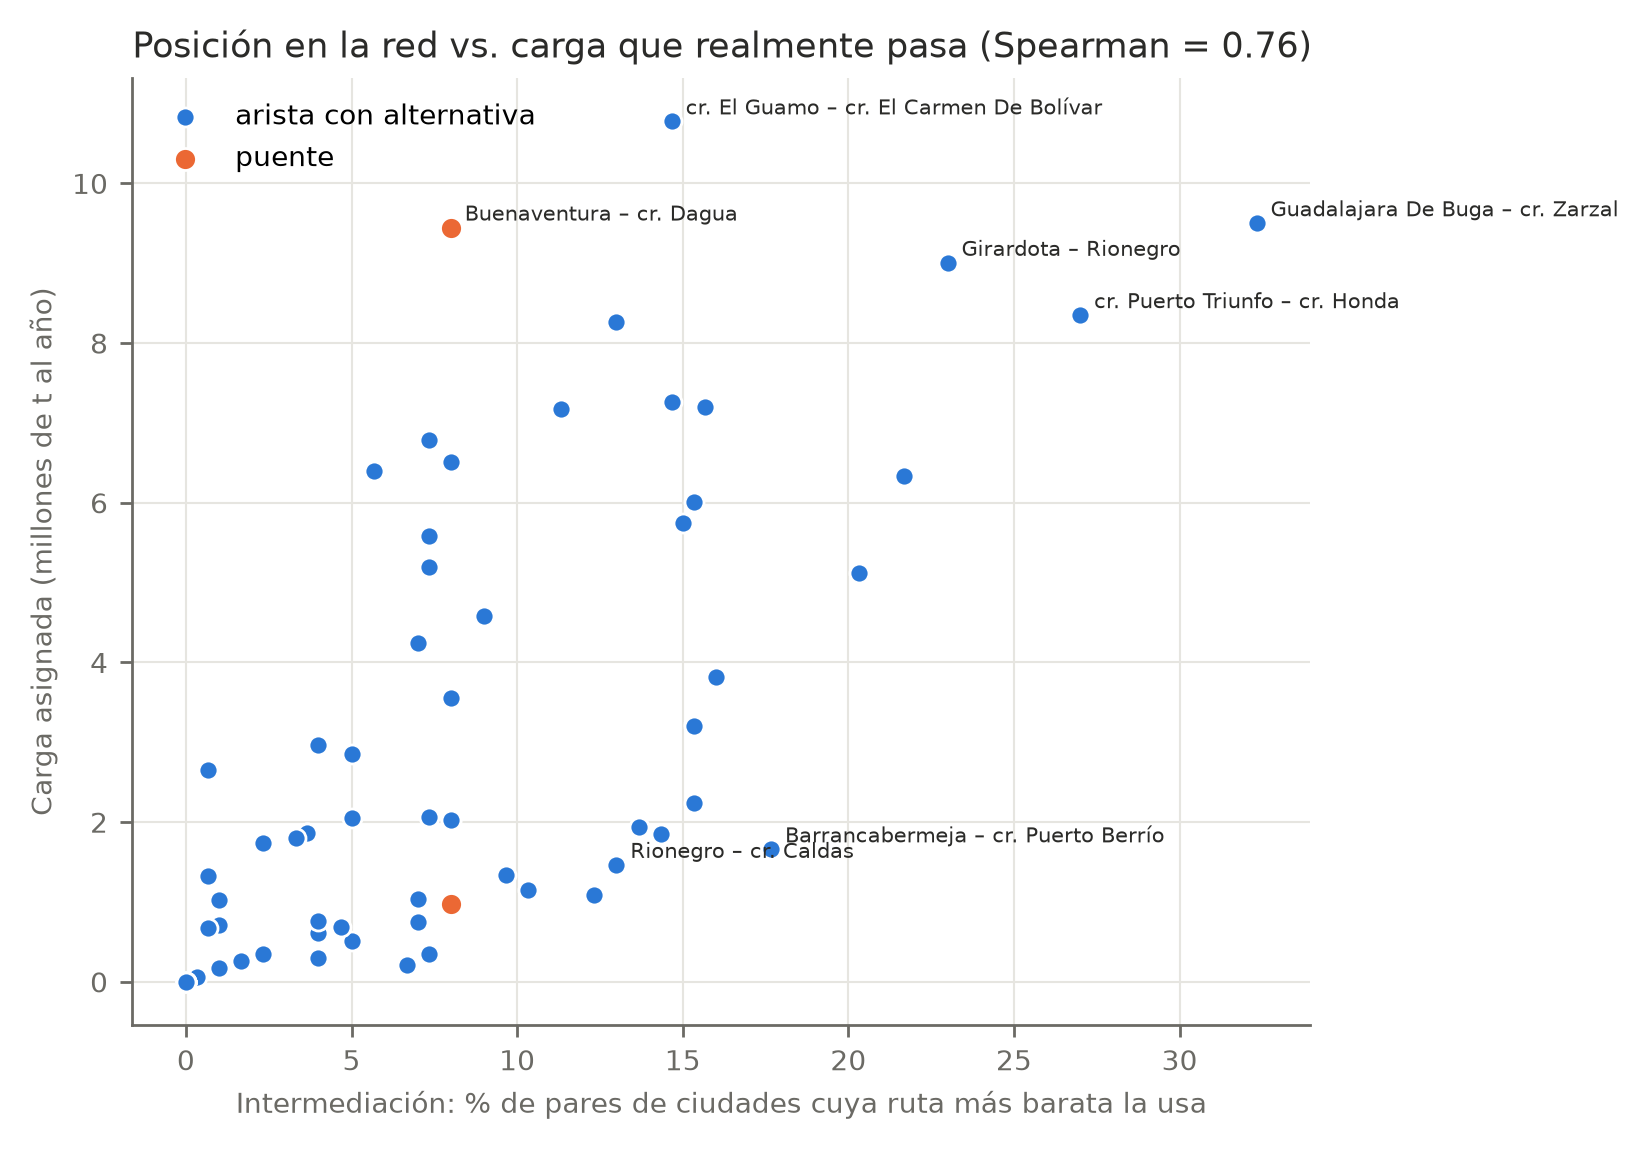
\includegraphics[width=\textwidth]{carga_vs_intermediacion.png}
    \column{0.42\textwidth}
      \begin{itemize}\small
        \item Spearman $\rho = 0{,}76$: se parecen, pero no ordenan igual
        \item \textbf{Subestimada:} Buenaventura--Dagua\\
              puesto 28 en posición, \alert{3 en carga} (21,6 \% de la carga)
        \item \textbf{Sobrestimada:} Barrancabermeja--Puerto Berrío\\
              puesto 6 en posición, 42 en carga
      \end{itemize}
  \end{columns}
\end{frame}

% 8 ------------------------------------------------
\begin{frame}{Resultado 2: el costo de cerrar}
  \begin{columns}[T]
    \column{0.42\textwidth}
      \textbf{Sin ruta (puentes)}\\[0.3em]
      \small
      Buenaventura--Dagua: \alert{9,45 Mt/año}\\
      Villavicencio--Puerto Gaitán: 0,98 Mt\\
      Sonsón--Rionegro: 0,97 Mt\\[0.8em]
      Por tramo de INVIAS, el acceso Puente Aurra--Medellín deja 8,14 Mt sin ruta.
    \column{0.56\textwidth}
      \textbf{Con desvío: mayor sobrecosto}\\[0.3em]
      \footnotesize
      \begin{tabular}{@{}lrr@{}}
        \toprule
        Arista & mil M COP/año & 14 días \\
        \midrule
        Buga--Zarzal & \alert{908,6} & 34,8 \\
        El Guamo--El Carmen & 687,3 & 26,4 \\
        Bosconia--Aguachica & 473,0 & 18,1 \\
        Ibagué--Zarzal & 383,9 & 14,7 \\
        Bogotá--Tocancipá & 327,2 & 12,6 \\
        \bottomrule
      \end{tabular}\\[0.6em]
      \small Buenaventura $\to$ Bogotá sin Buga--Zarzal: 470 $\to$ 821 km, por Cali y Neiva.
  \end{columns}
\end{frame}

% 9 ------------------------------------------------
\begin{frame}{Resultado 3: los tres ángulos y los tramos críticos}
  \begin{columns}[c]
    \column{0.55\textwidth}\centering
      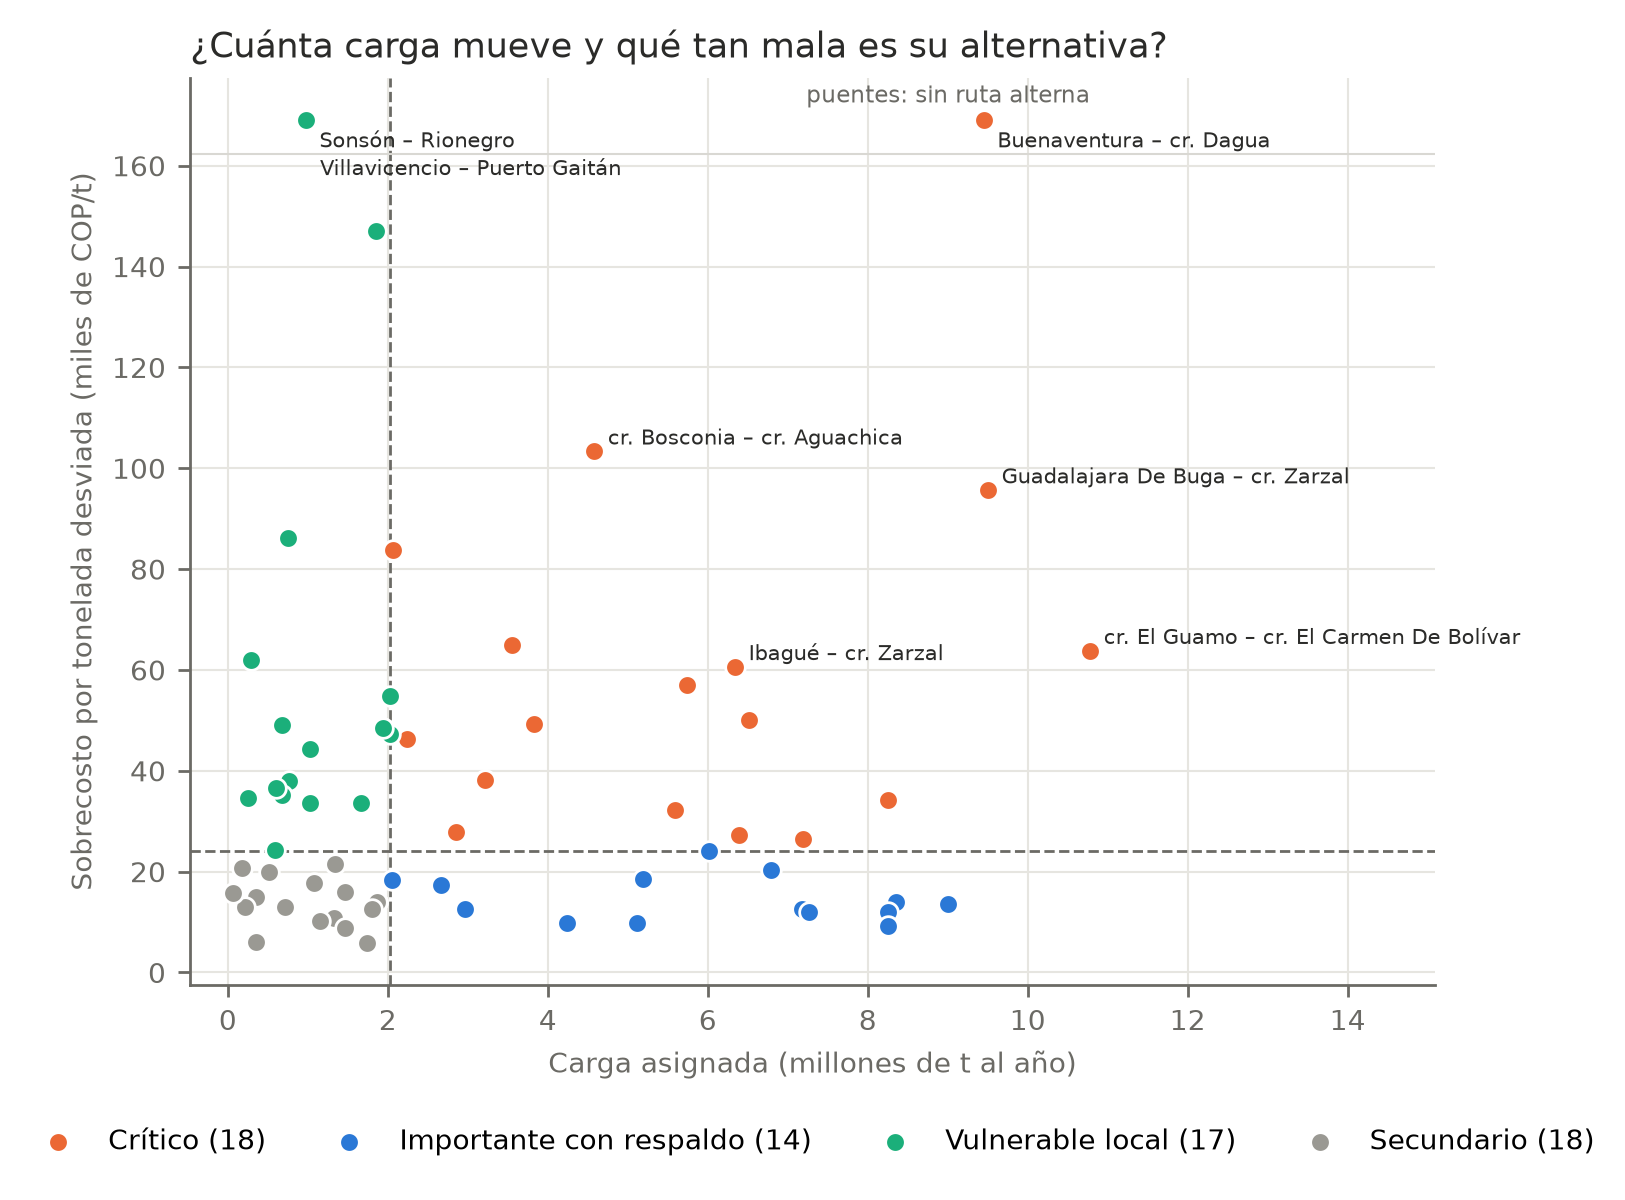
\includegraphics[width=\textwidth]{cuadrantes.png}
    \column{0.45\textwidth}
      \begin{itemize}\small
        \item Solo \alert{2 aristas} están en el top 10 de las tres medidas:
              Buga--Zarzal y Bogotá--Espinal
        \item Puerto Triunfo--Honda: puesto 2 en posición, \textbf{20} en sobrecosto
              (tiene un buen desvío)
        \item Bosconia--Aguachica: puesto 27 en posición, \textbf{3} en sobrecosto
        \item 18 críticas · 14 importantes con respaldo · 17 vulnerables locales ·
              18 secundarias · 10 sin carga
      \end{itemize}
  \end{columns}
\end{frame}

% 10 -----------------------------------------------
\begin{frame}{Demostración: la herramienta}
  \centering
  {\large Origen \quad + \quad destino \quad + \quad vías cerradas}\\[0.6em]
  $\Downarrow$\\[0.6em]
  {\large ruta alterna, km extra, sobrecosto en pesos, o ``no hay ruta''}\\[2em]
  \begin{columns}[T]
    \column{0.45\textwidth}
      \begin{block}{Caso 1}\small
        Buenaventura $\to$ Bogotá, cerrando Buga--Zarzal\\
        +350 km · +87.106 COP/t
      \end{block}
    \column{0.45\textwidth}
      \begin{block}{Caso 2}\small
        Buenaventura $\to$ Bogotá, cerrando Buenaventura--Dagua\\
        no hay ruta: 2,3 Mt/año
      \end{block}
  \end{columns}
\end{frame}

% 11 -----------------------------------------------
\begin{frame}{Conclusiones}
  \begin{itemize}
    \item \textbf{Más daño con desvío:} Buga--Zarzal, El Guamo--El Carmen,
          Bosconia--Aguachica.\\
          \textbf{Más daño sin ruta:} Buenaventura--Dagua (9,45 Mt/año).
    \item \textbf{La hipótesis se cumple:} posición, uso y consecuencia se parecen,
          pero no coinciden. El mapa solo no basta.
    \item \textbf{Lo crítico} es la combinación de mucha carga y una mala alternativa:
          18 aristas, una lista concreta para priorizar.
    \item \textbf{La red es frágil:} $\kappa = \lambda = 1$ y tres puentes.
  \end{itemize}
  \vspace{0.6em}
  \small\color{suave}
  Limitaciones: sin congestión (el sobrecosto es un mínimo), tarifa única, solo red
  primaria, datos de 2015, un cierre a la vez.
\end{frame}

% 12 -----------------------------------------------
\begin{frame}
  \centering
  {\Huge\bfseries Gracias}\\[1.5em]
  \large ¿Preguntas?\\[2em]
  \small\color{suave}
  Código, datos y herramienta: \texttt{github.com/gabrielsalcedo/graph-theory}
\end{frame}

\end{document}
